%%%%%%%%%%%%%%%%%%%%%%%%%%%%%%%%%%%%%%%%%%%%%%%%%%%%%%%%%%%%%%%%%%%%
%% I, the copyright holder of this work, release this work into the
%% public domain. This applies worldwide. In some countries this may
%% not be legally possible; if so: I grant anyone the right to use
%% this work for any purpose, without any conditions, unless such
%% conditions are required by law.
%%%%%%%%%%%%%%%%%%%%%%%%%%%%%%%%%%%%%%%%%%%%%%%%%%%%%%%%%%%%%%%%%%%%

\documentclass{beamer}
\usetheme[faculty=ped,basePath=../fibeamer,logo=../fibeamer/logo/mu/Logo-UC-3.png]{fibeamer}
\graphicspath{{../resources/}}

\usepackage{algorithm}
\usepackage{algpseudocode}

\usepackage[utf8]{inputenc}
\usepackage[
  main=english, %% By using `czech` or `slovak` as the main locale
                %% instead of `english`, you can typeset the
                %% presentation in either Czech or Slovak,
                %% respectively.
  czech, slovak %% The additional keys allow foreign texts to be
]{babel}        %% typeset as follows:
%%
%%   \begin{otherlanguage}{czech}   ... \end{otherlanguage}
%%   \begin{otherlanguage}{slovak}  ... \end{otherlanguage}
%%
%% These macros specify information about the presentation
\title{Ejercicios: funciones propias} %% that will be typeset on the
\subtitle{Semestre II-2026} %% title page.
\author{Profesora: Andreina Cota Vidaurre}
%% These additional packages are used within the document:
\usepackage{ragged2e}  % `\justifying` text
\usepackage{booktabs}  % Tables
\usepackage{tabularx}
\usepackage{tikz}      % Diagrams
\usetikzlibrary{calc, shapes, backgrounds}
\usetikzlibrary{positioning, arrows.meta, shadows.blur, shapes.geometric}
\usepackage{amsmath, amssymb}
\usepackage{url}       % `\url`s
\usepackage{listings}  % Code listings
\usepackage{graphicx}
\usepackage{amsmath}
\usepackage[T1]{fontenc}
\usepackage{xcolor}
\usepackage{minted}
% \usepackage{adjustbox}


% Definicion de pseudocodigo en espaniol
\lstdefinelanguage{PseudocodigoES}{
    morekeywords={INICIO,FIN,PARA,HACER,SI,ENTONCES,FIN_SI,FIN_PARA,IMPRIMIR},
    sensitive=true,
    morecomment=[l]{//},
    morestring=[b]"
}

% Definicion de pseudocodigo en ingles
\lstdefinelanguage{PseudocodeEN}{
    morekeywords={BEGIN,END,FOR,DO,IF,THEN,END_IF,END_FOR,PRINT},
    sensitive=true,
    morecomment=[l]{//},
    morestring=[b]"
}

\lstset{
    basicstyle=\ttfamily\small,
    keywordstyle=\bfseries,
    columns=fullflexible,
    keepspaces=true,
    showstringspaces=false,
    frame=single,
    xleftmargin=0em,
    framexleftmargin=0em,
    framesep=2pt,
    gobble=4,
    resetmargins=true,
    aboveskip=0pt,
    belowskip=0pt
}

\lstdefinestyle{pythonstyle}{
    language=Python,
    basicstyle=\ttfamily\small,
    keywordstyle=\bfseries,
    commentstyle=\itshape,
    stringstyle=\ttfamily,
    showstringspaces=false,
    columns=fullflexible,
    keepspaces=true,
    frame=single,
    breaklines=true,
    xleftmargin=0em,
    framexleftmargin=0em,
    framesep=2pt,
    aboveskip=0pt,
    belowskip=0pt,
    gobble=4,
    resetmargins=true,
    emph={print,input,int,float,str,bool,len,range},
    emphstyle=\bfseries
}

\lstset{style=pythonstyle}

% Estilos del diagrama
\tikzstyle{iniciofin} = [
    ellipse,
    minimum width=2.5cm,
    minimum height=1cm,
    text centered,
    draw=black,
    fill=blue!25
]

\tikzstyle{proceso} = [
    rectangle,
    rounded corners,
    minimum width=3cm,
    minimum height=1cm,
    text centered,
    draw=black,
    fill=cyan!20
]

\tikzstyle{decision} = [
    diamond,
    aspect=2,
    text centered,
    draw=black,
    fill=yellow!35
]

\tikzstyle{flecha} = [
    thick,
    ->,
    >=Stealth
]

% \definecolor{green_python}{HTML}{52A736}

% \newcolumntype{Y}{>{\raggedright\arraybackslash}X}

\frenchspacing
\begin{document}
  \shorthandoff{-}
  \frame[c]{\maketitle}

% \begin{darkframes}

    % \begin{frame}[fragile,t]{Validar y limpiar un mensaje de radio}
    %     En comunicaciones militares, los mensajes de radio suelen llegar con espacios extra, caracteres en mayúsculas y minúsculas mezcladas, y palabras clave que deben verificarse. El sistema debe limpiar el mensaje y analizarlo antes de procesarlo.
        
    %      Definir una función que reciba un mensaje de radio como string y realice las siguientes operaciones:
    %     \begin{itemize}
    %         \item Eliminar espacios al inicio y al final del mensaje
    %         \item Contar cuántas veces aparece la palabra "ALFA"
    %         \item Determinar si contiene la palabra "URGENTE"
    %         \item Mostrar la longitud del mensaje ya limpio
    %     \end{itemize}
    % \end{frame}

    % \begin{frame}[fragile,t]{Validar y limpiar un mensaje de radio}
    %     \begin{minted}[xleftmargin=-2cm, frame=leftline, fontsize=\small]{python}
    %     # Resultado esperado:
    %     analizar_mensaje("  ALFA uno URGENTE ALFA tres ALFA  ")
        
    %     # Mensaje limpio: 'ALFA uno URGENTE ALFA tres ALFA'
    %     # Longitud: 31 caracteres
    %     # Apariciones de 'ALFA': 3
    %     # Contiene 'URGENTE': Si, en posicion 14
    %     \end{minted}
    % \end{frame}

    % \begin{frame}[fragile,t]{Análisis métrico de "Gracias a la vida"}
    %     \begin{figure}
    %         \centering
    %         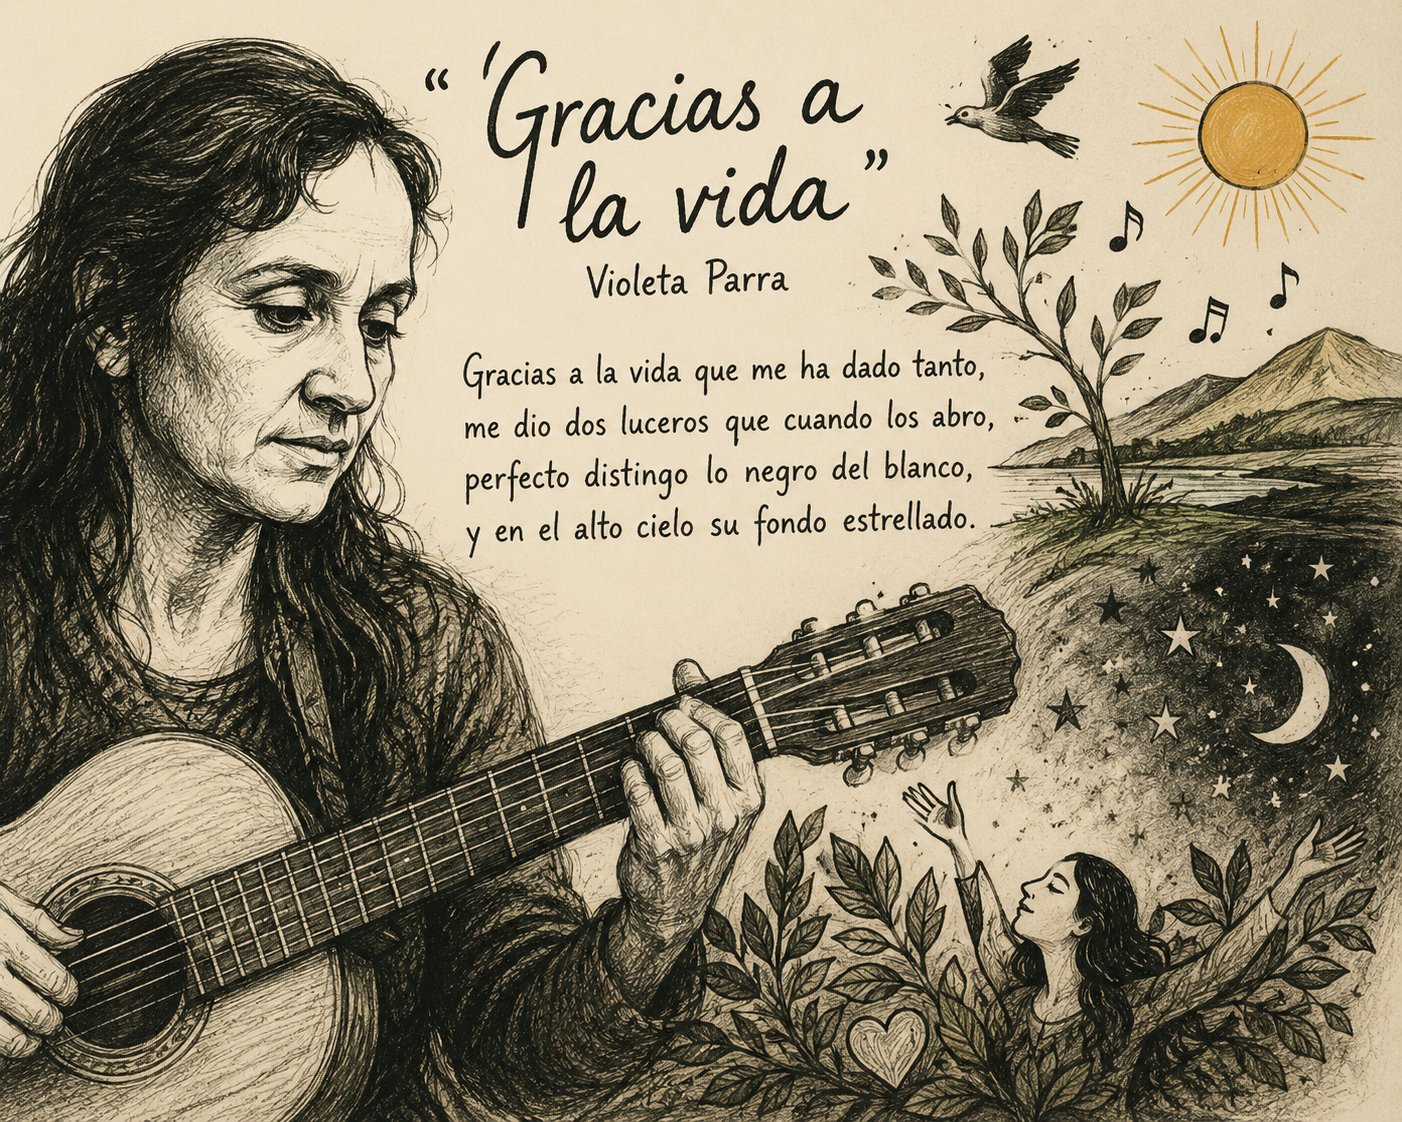
\includegraphics[width=0.4\linewidth]{violera_parra.png}
    %     \end{figure}
    %     Dado el siguiente fragmento de la primera estrofa de "Gracias a la vida", definir una función que reciba el texto como string y calcule:
    %     \begin{itemize}
    %         \item Total de palabras del fragmento de la canción
    %         \item Contar cuántas veces se repite la palabra "vida"
    %         \item Determinar si el verso comienza con la palabra "Gracias"
    %     \end{itemize}
    % \end{frame}

    % \begin{frame}[fragile,t]{Análisis métrico de "Gracias a la vida"}
    %     \begin{minted}[xleftmargin=-2cm, frame=leftline, fontsize=\small]{python}
    %         """Gracias a la vida, que me ha dado tanto
    %         Me ha dado la marcha de mis pies cansados
    %         Con ellos, anduve ciudades y charcos
    %         Playas y desiertos, montañas y llanos
    %         Y la casa tuya, tu calle y tu patio.
    %         """
    %     \end{minted}
    % \end{frame}

    \begin{frame}[fragile,t]{Área y perímetro de un trapecio}
        \begin{figure}
            \centering
            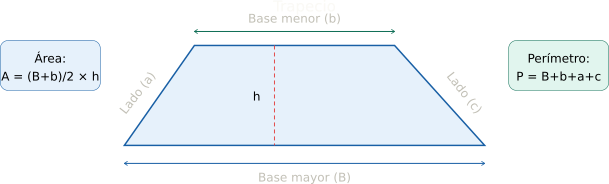
\includegraphics[width=\linewidth]{trapecio_geometria.png}
        \end{figure}
        \begin{minted}[xleftmargin=-2cm, frame=leftline, fontsize=\small]{python}
        def calcular_area_trapecio(base_mayor, base_menor, altura):
            area = (base_mayor + base_menor) / 2 * altura
            return area
        \end{minted}
        \begin{minted}[xleftmargin=-2cm, frame=leftline, fontsize=\small]{python}
        def calcular_perimetro_trapecio(base_mayor, base_menor, a, c):
            perimetro = base_mayor + base_menor + a + c
            return area
        \end{minted}
    \end{frame}

    
    \begin{frame}[fragile, t]{Área y perímetro de una elipse}
        \begin{figure}
            \centering
            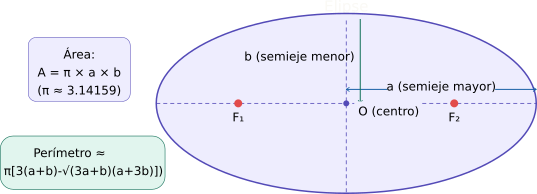
\includegraphics[width=0.5\linewidth]{ellipse_geometria.png}
        \end{figure}
        \begin{minted}[xleftmargin=-2cm, frame=leftline, fontsize=\small]{python}
        def calcular_perimetro_elipse_ramanujan(a, b):
            calculo = ((3 * a) + b) * (a + (3 * b))
            raiz = math.sqrt(calculo)
            perimetro = math.pi * ((3 * (a + b)) - raiz)
            return perimetro
        \end{minted}
        \begin{minted}[xleftmargin=-2cm, frame=leftline, fontsize=\small]{python}
        def calcular_area_elipse(a, b):
            return math.pi * a * b
        \end{minted}
    \end{frame}

    \begin{frame}[fragile, t]{Área y perímetro del hexágono regular}
        \begin{figure}
            \centering
            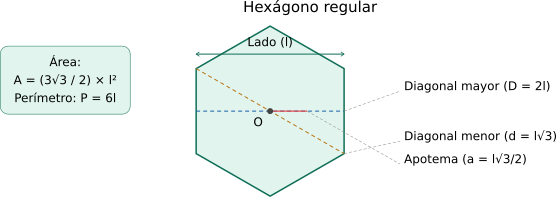
\includegraphics[width=0.5\linewidth]{hexagono_geometria.png}
        \end{figure}
        \begin{minted}[xleftmargin=-2cm, frame=leftline, fontsize=\small]{python}
        def calcular_perimetro_hexagono(lado):
            # escribir el cuerpo del codigo
            pass    
        \end{minted}
        \begin{minted}[xleftmargin=-2cm, frame=leftline, fontsize=\small]{python}
        def calcular_area_hexagono(lado):
            # escribir el cuerpo del codigo
            pass    
        \end{minted}
    \end{frame}

    \begin{frame}[fragile, t]{Área y perímetro del pentágono regular}
        \begin{figure}
            \centering
            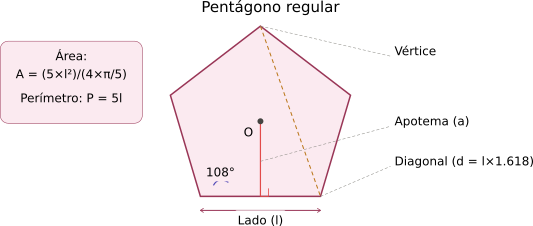
\includegraphics[width=0.5\linewidth]{pentagono_geometria.png}
        \end{figure}
        \begin{minted}[xleftmargin=-2cm, frame=leftline, fontsize=\small]{python}
            def calcular_perimetro_pentagono(lado):
                # escribir el cuerpo del codigo
                pass    
        \end{minted}
        \begin{minted}[xleftmargin=-2cm, frame=leftline, fontsize=\small]{python}
            def calcular_area_pentagono(lado):
                # escribir el cuerpo del codigo
                pass    
        \end{minted}
    \end{frame}

    \begin{frame}[fragile, t]{Año bisiesto}
        Definir una función que reciba un año y determine si es bisiesto o no. Un año es bisiesto si es divisible por 4, excepto los años centenarios, a menos que también sean divisibles por 400.
        \begin{minted}[xleftmargin=-2cm, frame=leftline, fontsize=\small]{python}
            # Resultado esperado:
            # es_bisiesto(2024) → "2024 es bisiesto"
            # es_bisiesto(1900) → "1900 NO es bisiesto"
            # es_bisiesto(2000) → "2000 es bisiesto"
        \end{minted}
    \end{frame}

    \begin{frame}[fragile, t]{Copa Mundial}
        \begin{figure}
            \centering
            
\includegraphics[width=0.2\linewidth]{copa_mundial_2026.png}
        \end{figure}
        La Copa Mundial de la FIFA se celebra cada 4 años. La última edición antes del año 2000 fue en 1998, por lo que los años válidos siguen el patrón: 1998, 2002, 2006, 2010...
        
         Definir una función que reciba un año como argumento y determine si ese año se celebra la Copa Mundial de la FIFA. Para considerarse válido, el año debe ser 1998 o posterior y cumplir el patrón de cada 4 años.
    \end{frame}

    \begin{frame}[fragile, t]{Copa Mundial}
        \begin{minted}[xleftmargin=-2cm, frame=leftline, fontsize=\small]{python}
            # Resultados esperados:
            mundial(2026)  # "¡Sí! En 2026 se celebra la Copa Mundial."
            mundial(2025)  # "No. En 2025 no hay Copa Mundial."
            mundial(1990)  # "Año fuera del rango válido. 
                           # Ingrese un año desde 1998 en adelante."
        \end{minted}
    \end{frame}

    \begin{frame}[fragile, t]{Velocidad angular de una rueda}
        Una rueda gira a cierta cantidad de RPM (revoluciones por minuto). Definir una función que reciba las RPM y retorne la velocidad angular en radianes por segundo. Fórmula: \[\omega = \frac{2\pi \times RPM}{60}\]
        \begin{minted}[xleftmargin=-2cm, frame=leftline, fontsize=\small]{python}
            # Resultado esperado:
            # velocidad_angular(120) → 12.566 rad/s
            # velocidad_angular(3000) → 314.159 rad/s
        \end{minted}
    \end{frame}

    % \begin{frame}[fragile, t]{Simulador de lanzamiento de dados}
    %     \begin{figure}
    %         \centering
    %         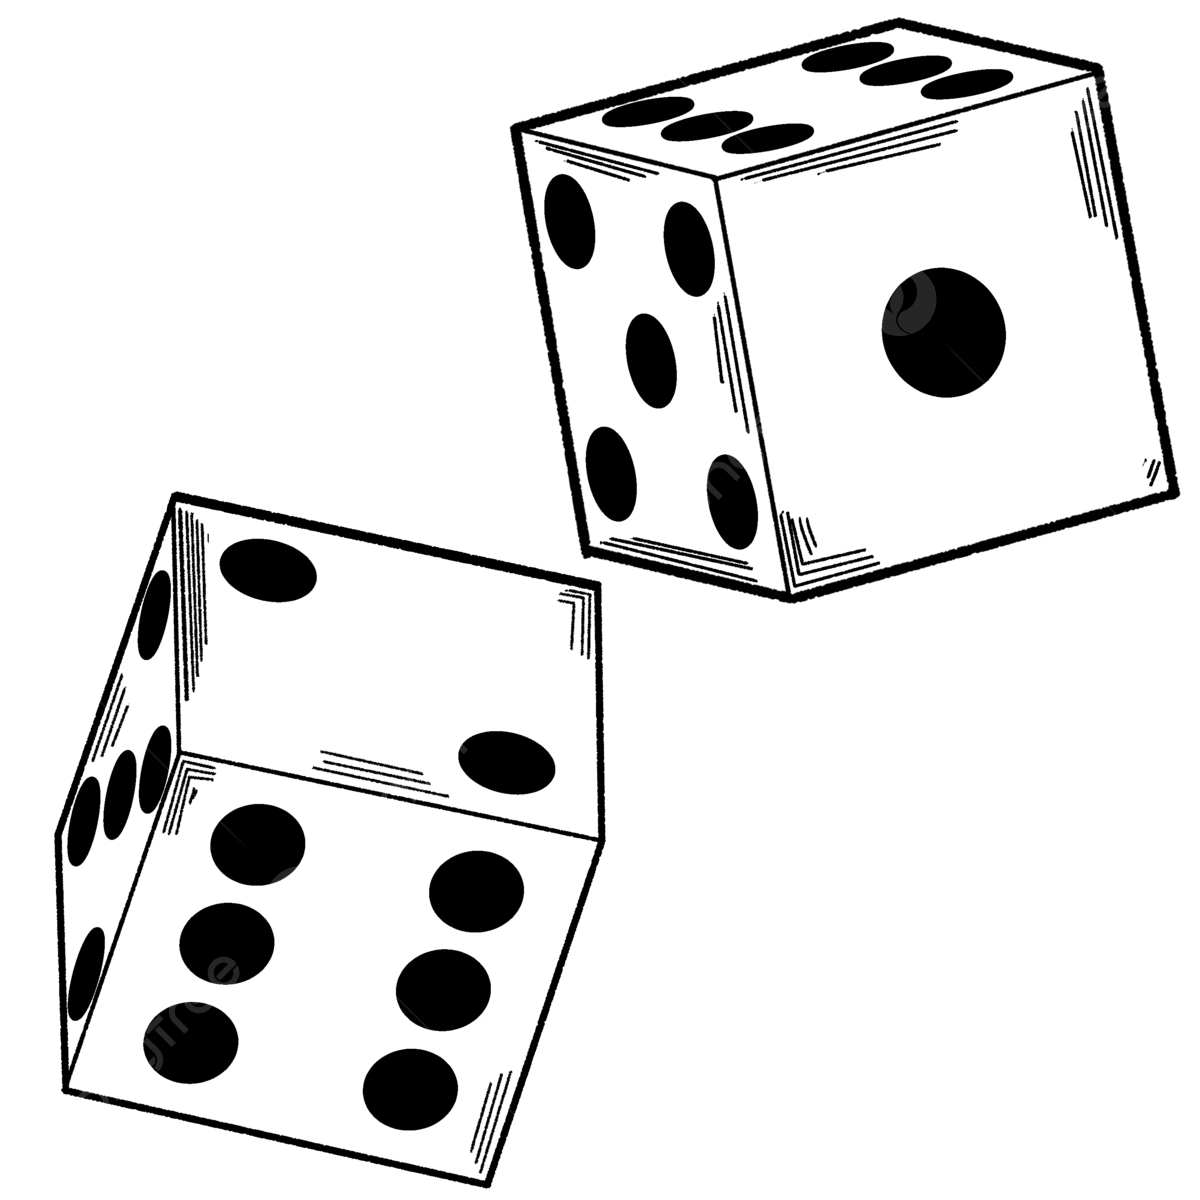
\includegraphics[width=0.2\linewidth]{dados.png}
    %     \end{figure}
    %     En varios juegos de mesa, el resultado de dos dados determina el movimiento del jugador. Ciertos valores tienen consecuencias especiales: si ambos dados muestran el mismo número (doble), el jugador vuelve a lanzar; si la suma es 7, pierde un turno.
        
    %     Definir una función que reciba el nombre del jugador, simule el lanzamiento de dos dados de 6 caras y retorne un mensaje indicando la suma obtenida y si ocurrió algún evento especial.
    % \end{frame}

    %     \begin{frame}[fragile, t]{Simulador de lanzamiento de dados}
    %     \begin{minted}[xleftmargin=-2cm, frame=leftline, fontsize=\small]{python}
    %         # Resultados esperados (los valores varían por ser aleatorios):
    %         lanzar_dados("Ana")
    %         # Ana lanzó: 3 + 3 = 6 → ¡Doble! Lanza de nuevo.
            
    %         lanzar_dados("Carlos")
    %         # Carlos lanzó: 4 + 3 = 7 → Mala suerte, pierdes un turno.
            
    %         lanzar_dados("Pedro")
    %         # Pedro lanzó: 2 + 5 = 7 → Mala suerte, pierdes un turno.
            
    %         lanzar_dados("Ana")
    %         # Ana lanzó: 1 + 4 = 5 → Avanza 5 casillas.
    %     \end{minted}
    % \end{frame}

    % \begin{frame}[fragile, t]{Simulación de precisión de tiro}
    %     \begin{figure}
    %         \centering
    %         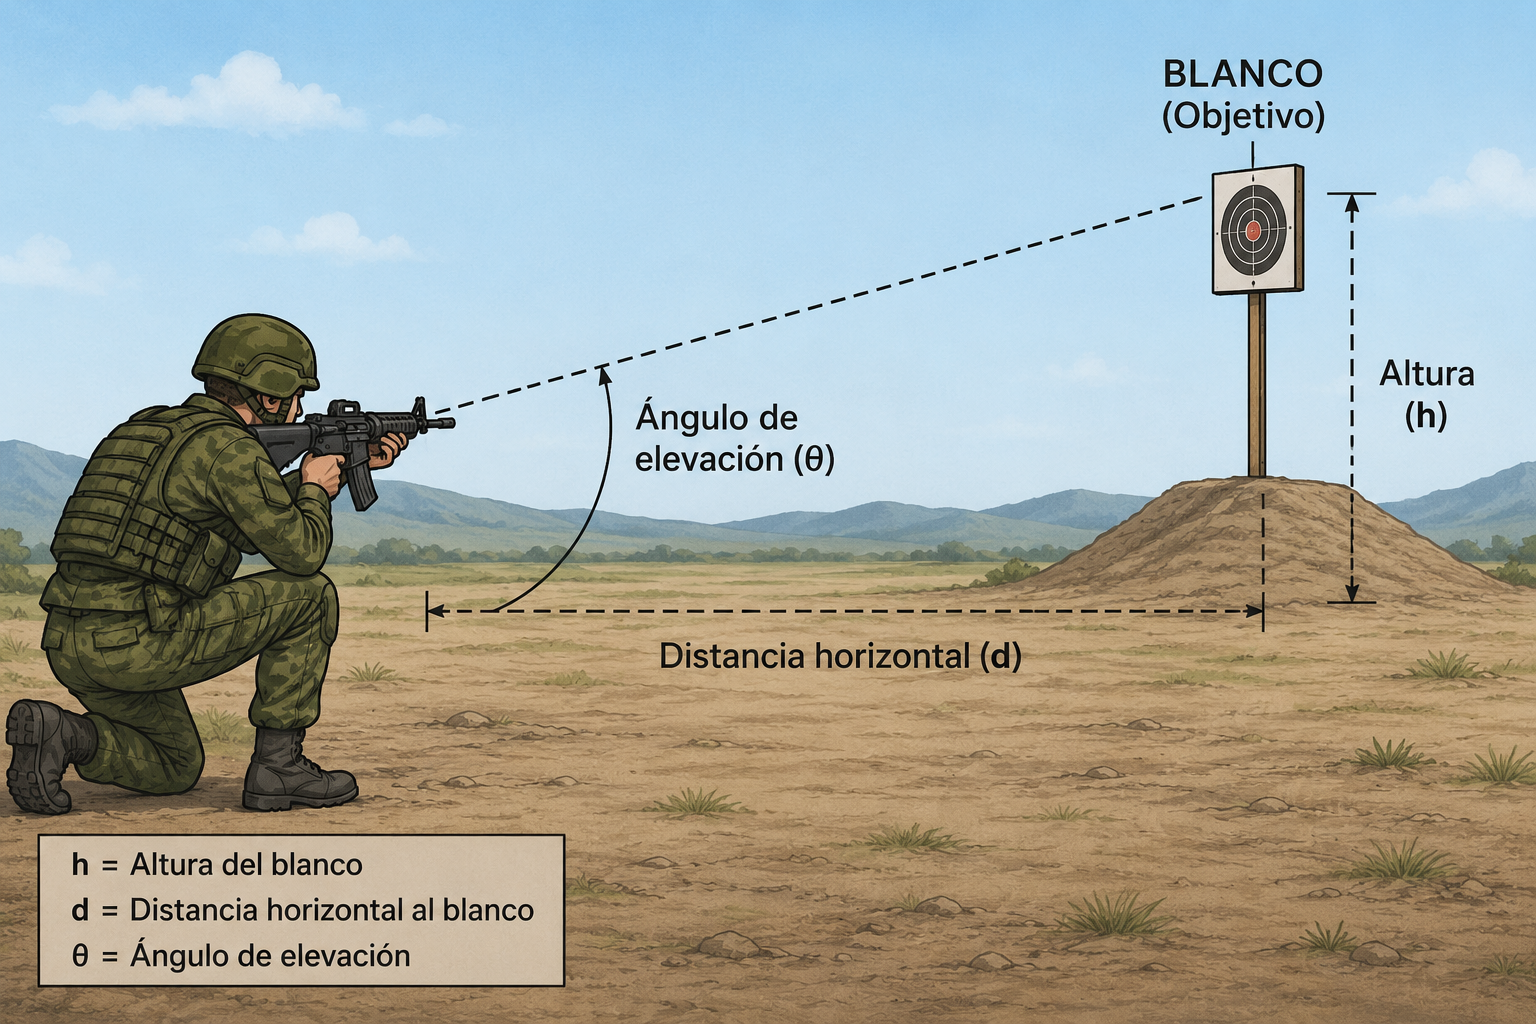
\includegraphics[width=0.45\linewidth]{soldado_tiro_blanco.png}
    %     \end{figure}
    %     Un soldado realiza 5 disparos al blanco. Cada disparo tiene una probabilidad aleatoria de impacto (entre 0 y 100). Si el valor supera 60, se considera un acierto. La función debe contar los aciertos y determinar si el soldado aprueba la prueba de tiro (mínimo 3 de 5).
        
    %      Definir una función que reciba el nombre del soldado y simule su prueba de tiro, reportando cada disparo y el resultado final.
    % \end{frame}

    % \begin{frame}[fragile, t]{Simulación de precisión de tiro}
    %     \begin{minted}[xleftmargin=-2cm, frame=leftline, fontsize=\small]{python}
    %         # Resultado esperado (varía por ser aleatorio):
    %         prueba_de_tiro("Soldado Vega")
    %         # Soldado Vega — Prueba de tiro:
    %         #   Disparo 1: 74 → Acierto
    %         #   Disparo 2: 38 → Fallo
    %         #   Disparo 3: 91 → Acierto
    %         #   Disparo 4: 55 → Fallo
    %         #   Disparo 5: 83 → Acierto
    %         # Resultado: APROBADO (3/5 aciertos)
    %     \end{minted}
    % \end{frame}

\end{document}
